\RequirePackage{lineno}
\documentclass[a4paper,11pt]{article}
\linenumbers

\usepackage{xcolor}
%\usepackage{wrapfig}
\usepackage{graphicx}
%\usepackage{multirow}
%\usepackage{array}
%\usepackage{xspace}
%\usepackage{ifthen}
\usepackage{times}

%\usepackage{geometry}
% \geometry{
% a4paper,
% total={170mm,257mm},
% left=15mm,
% right=15mm,
% top=30mm,
% bottom=22mm,
% }

%\usepackage{lastpage}
%\usepackage{fancyhdr}
%\pagestyle{fancy}
%\footskip 20pt
%\fancyhf{}
%\chead{Report Referee 2}
%\cfoot{{Page \thepage~of~\pageref{LastPage}}}
%\renewcommand{\headrulewidth}{0.0pt}
%\renewcommand{\footrulewidth}{0.0pt}

\begin{document}
%\fontsize{10}{12}
%\selectfont


\section*{Report from referee 2 JPG}

This work by Kumar, Shukla, and Bhattacharyya presents a phenomenological study of 
quarkonia (J/psi and Upsilon) suppression in PbPb collisions at  5.02 TeV. 
The predictions of their phenomenological model --including gluon-dissociation 
inside the QGP, suppression due to hadronic comovers, regeneration of heavy-quark 
pairs, and nuclear parton distribution functions (nPDFs) effects-- are compared 
to the experimental data from ALICE, ATLAS, and CMS. The model reproduces the 
experimental pT and centrality dependencies of the observed J/psi and Upsilon 
suppressions, except for the larger observed suppression of J/psi at pT > 10 GeV. 
The paper conveys interesting information, and I do not see any obvious flaw in 
their theoretical implementation of the different effects included. However, 
before I can recommend acceptance the following issues should be clarified:
\newline



%Dear Editor,
%We would like to thank the referee for reviewing this paper and furnishing the report.
%We have carefully considered all comments, and we have applied the corresponding changes to the original
%version of the paper to address the issues raised. Detailed responses to all the comments made by referee
%can be found below. We are at your disposal for any further clarifications and/or additional information.

{\color{blue}
We would like to thank the referee for reviewing this paper and furnishing the report.
Detailed responses to all the comments made by referee can be found below.}


\begin{enumerate}

\item There is no discussion of the different contributions and suppression 
mechanisms for prompt/feed-down J/$\psi$ mesons. This is a key element, considered 
in the Upsilon case, but not in the J/$\psi$ case.

{\color{red} The feed-down contributions for the J/$\psi$ are not very large.
  At the LHC energies around 80\% J/$\psi$ are from the directly produced hard
  scattering~\cite{Lansberg:2019adr}. Moreover, the gluon dissociation cross section for
  the excited charmonia states are not reliable. Thus we chose to not consider the feed-down
  from the higher states for the J/$\psi$. 
} 

\item There is no explanation of how the authors take into account in their model 
the different (central and forward) rapidities of the quarkonia measurements. 
It seems that they fix their entropy density to the total charged particle density 
measured in the top 0-5$\%$ most central PbPb collisions, dNch/deta=1943, but 
nothing is said on how the rapidity dependence of this multiplicity is 
taken into account in the modeling of their medium density. 

{ \color{blue} The initial temperature is estimated using the measured charged particle
  multiplicity. The charged particle multiplicity is different for different
  rapidity regions. For forward rapidities we use ALICE measurement~\cite{Adam:2016ddh}
  of charged particle density 1640 which gives the initial temperature for $\tau_0$=0.3 fm
  as 0.487 GeV. This information is updated in the paper.
}







\item The symbols convention is not always clear. E.g. the authors use "Q" and 
"q" as subindices for the same object (heavy quark) quantities. The use "M", 
"m", m$_q$", "m$_Q$" for the same quantity (heavy-quark mass). They should check 
all parameters and expressions and uniformize them. 

{ \color{blue} In the paper the symbol $M_Q$ is used for Quarkonium mass and $m_q$ is used for
  heavy quark mass.}

\end{enumerate}


- Page 2 line 9: - transition towards a quark-gluon plasma (QGP) state in which . \newline 
- {\color{blue} done} \newline

- Page 2 line 20: quarkonia \newline
- {\color{blue} done} \newline

- Page 2 has increases $\rightarrow$ has increased
- {\color{blue} done} \newline

- Page 3 line 10: J/psis -> J/psi mesons \newline
- {\color{blue} done} \newline

- Page 3 where both a \newline
- {\color{blue} done} \newline

- measurement of the same at the CMS \newline
- {\color{blue} modified} \newline

field has attracted 
- {\color{blue} modified} \newline

 with the surrounding gluons 
 - {\color{blue} modified} \newline
 
* Page 4: \newline

 Define key 'rhog' parameter in the text. \newline 
- {\color{blue} done} \newline
 in the color dipole ... \newline
- {\color{blue} done}\newline

* Page 5: \newline

 Eq 5 $\rightarrow$ Eq. (5) \newline

* Page 6: \newline

Captions Figs. 2, 3: Specify that the pT refers to the J/psi (not gluon) pT 
- {\color{blue} done}\newline

%%%%%%%%%%%%%%%%%%%%%%%%%%%%%%%%%%%%%%%%%%%%%%%%%%%%%%%%%%%%%%%%%%%%%%%%%%%%%%%%%%%%%%%%%%%
Eq. (6): Explicitly define s, MQ in the text. \newline

%{\color{red} where $M_{Q}$ is the mass of quarkonia and $s$ is the centre of mass energy of
%of the quarkonium-gluon system. (note done yet as I am not sure.)}

{\color{blue}  In the paper now we modify the texts after Eq. 5. 
where $\sigma_{D}(s) = \sigma_{D}(q^0(s))$ in terms of the square of the center of
mass energy $s$ of the quarkonium-gluon system given by
$s=M_{Q}^{2} + 2  p_g \, \sqrt{M_{Q}^2 + p^2} - 2  p_g \, p \, {\rm cos\theta}$.
Here $M_{Q}$ is the mass and $p$ is the momentum of quarkonium and $\theta$ is the angle
between the quarkonium and the gluon.
  The variables $q^0$ and $s$ are related by $q^{0} = (s-M_{Q}^{2})/(2\,M_{Q})$. 
$v_{\rm rel}$ is the relative velocity between the quarkonium and the gluon~\cite{Kumar:2014kfa}.
  The formula in Eq. 5 is assumed
for the most central collisions. We multiplied by a system size dependent factor
($\sqrt{N_{\rm part}/2A}$) to get the dissociation rate for other centralities. \newline

we modify the texts after Eq. 7. \newline

The variable $s$ is the square of center of mass energy between the two heavy quarks with
energy-momenta ($E_1$, ${\rm\bf p_1}$) and ($E_2$, ${\rm\bf p_2}$) with $v_{\rm rel}$ as their
relative velocity.

The functions $f_{q/\bar{q}}(p)$ are taken as normalized near-thermal distribution functions
of $q/\bar{q}$. These distributions can be described by the Tsallis
function as follows 
\begin{equation}
f_{q} (p,T) = A_{n}\,\left( 1+\frac{ \sqrt{p^2+m_q^2} }{n \,T} \right)^{-n}.
\end{equation}
Here $A_n$ is the normalization factor and $n=12$ is obtained by fitting the
transverse momentum spectra of D mesons measured by CMS experiment.
}
%%%%%%%%%%%%%%%%%%%%%%%%%%%%%%%%%%%%%%%%%%%%%%%%%%%%%%%%%%%%%%%%%%%%%%%%%%%%%%%%%%%%%%%%%%%%

What is the motivation for the Tsallis function fit of Eq. (8)? Provide 
a reference for the n = 14 parameter choice. 

{\color{blue} Here we add a figure and the following revision in the paper.

  Since the heavy quarks produced are not fully thermalized in the medium
  we use near thermal distributions given by Tsallis function.
  (There was a typo, we used $n=12$ in the work.)
  Figure 3 gives the transverse momentum spectra of D mesons in pp and PbPb collisions
  at $\sqrt{s_{\rm NN}}=5.02$ TeV measured by CMS experiment. The spectra are fitted
  by Tsallis function with $n=6.9$ for pp and $n=12$ for PbPb collisions.
}

\begin{figure}
  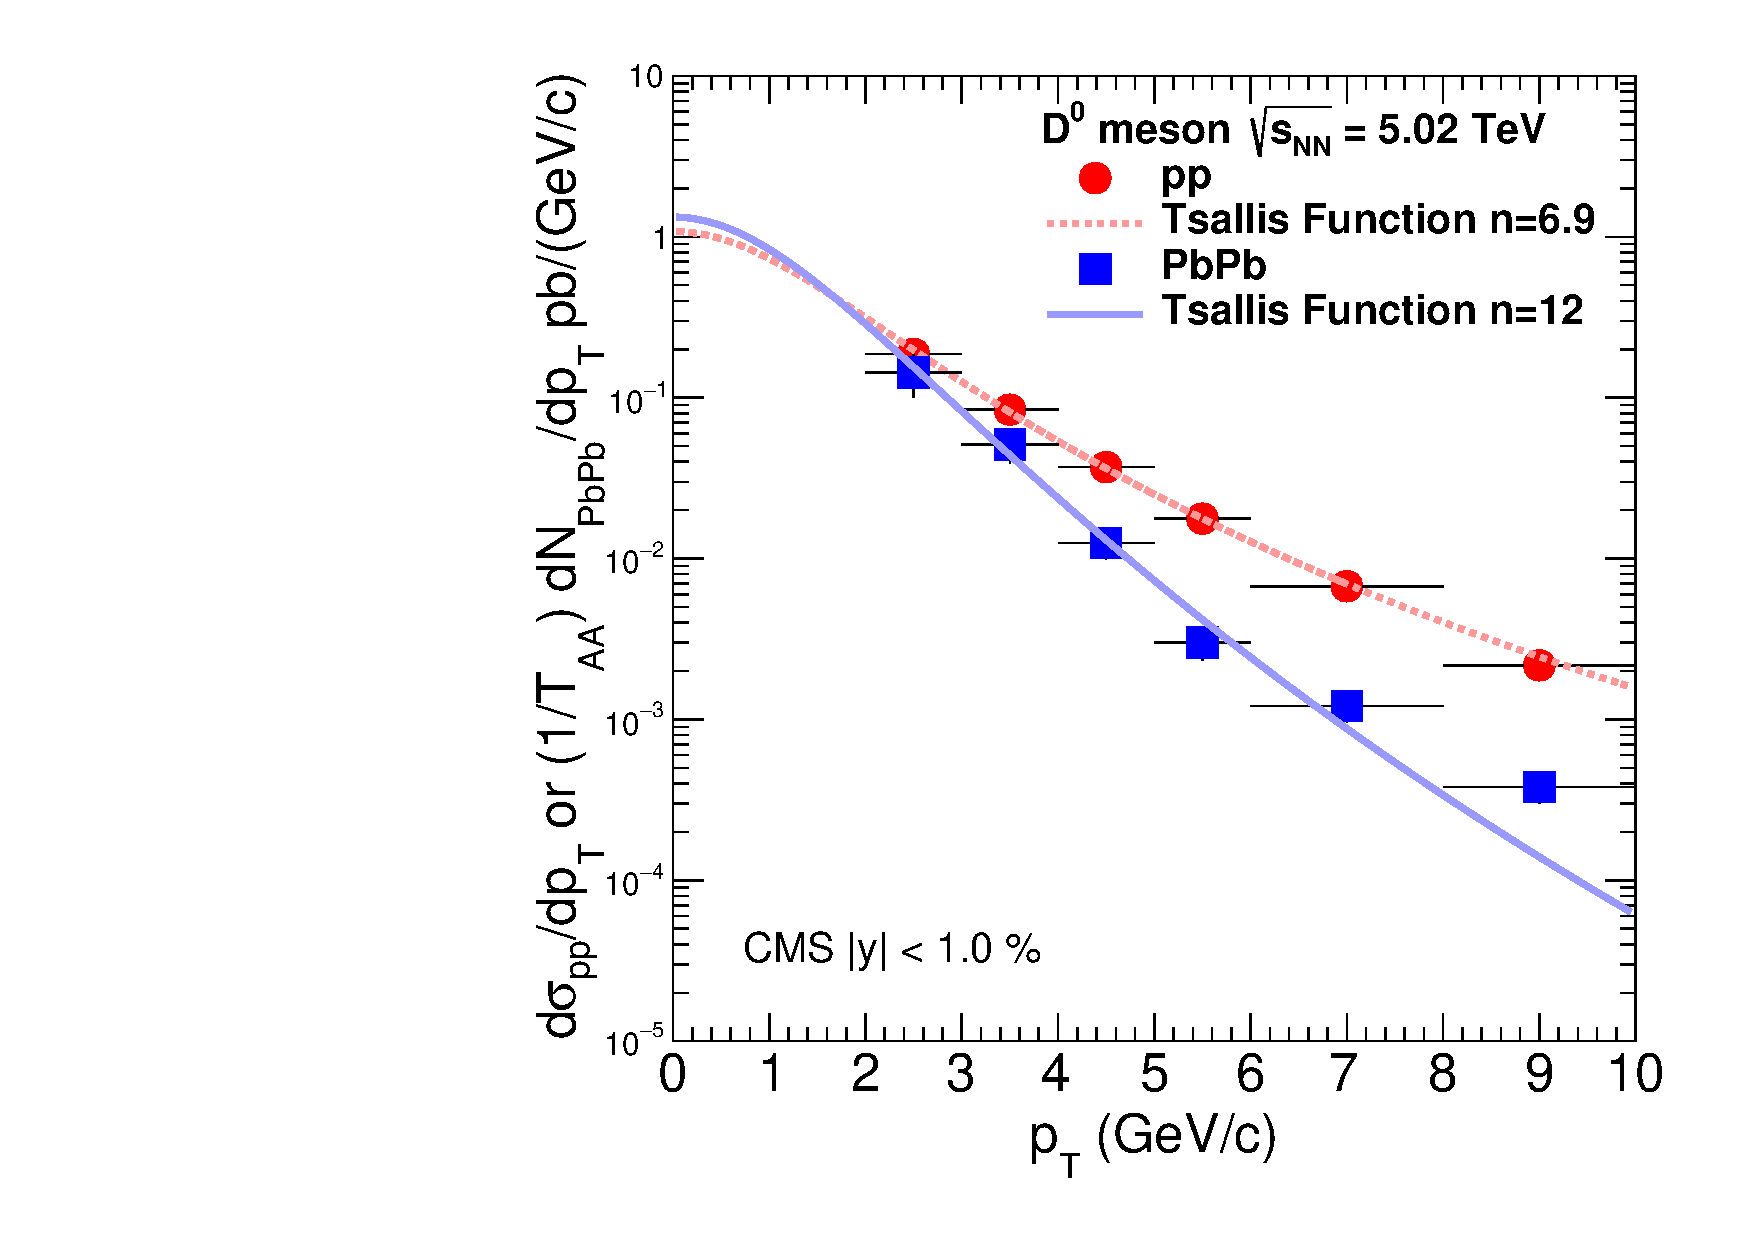
\includegraphics[width=0.60\textwidth]{Figure3_DMeson_502TeV.pdf}
  \caption{The transverse momentum spectra of D mesons in pp and PbPb collisions
    at $\sqrt{s_{\rm NN}}=5.02$ TeV measured by CMS experiment \cite{Sirunyan:2017xss}.
    The spectra are fitted
    by Tsallis function withb$n=6.9$ for pp and $n=12$ for PbPb collisions.
  }
  \label{fig:Figure_Tsallis}
\end{figure}

%%%%%%%%%%%%%%%%%%%%%%%%%%%%%%%%%%%%%%%%%%%%%%%%%%%%%%%%%%%%%%%%%%%%%%%%%%%%%%%%%%%%%%%%%%%


* Page 7: 

Eqs. (9), (10): 'Ncoll' is left completely undefined.
- {\color{blue} done}\newline

total final hadron multiplicity 
- {\color{blue} done}\newline
* Page 8: 

Please write down the numerical value of the c.m.-energy-independent factors obtained 
from the color evaporation model that they use to relate the heavy-quark and quarkonia 
cross sections. 

- {\color{red} The quarkonium production cross sections are calculated from the measured heavy quark
  production cross-section using the energy independent factors (0.00526 for J/$\psi$ and 0.002 for $\Upsilon$)
  obtained from the color evaporation model [26, 62, 63]}\newline

* Page 9: 

Typo 'quamtity' [run spell-check] 
- {\color{blue} done}\newline

Uniformize style: "Fig. X(a)" or "Fig. X (a)", consistently throughout the text. 
- {\color{blue} done}\newline
* Page 11: 

for the ALICE 
- {\color{blue} done}\newline
... a trend that ... 
- {\color{blue} done}\newline
* Page 12: 

kinetic $\rightarrow$ kinematic 
- {\color{blue} done}\newline

Move the last line of the page "The states Upsilon(1S)... bound states." to 
the text right before Eqs. (14)--(16). As of now there is a gap, discussing 
other issues, between this sentence and its associated relevant text later on. 
- {\color{blue} done}\newline
* Page 14: 

fis $\rightarrow$ is 
- {\color{blue} done}\newline
* Page 15: 

due to gluons in the QGP $\rightarrow$ due to gluon dissociation in the QGP 
[Note that the authors suggest that heavy-quark energy loss could explain 
the difference, and this would be also "due to gluons".]
- {\color{blue} done}\newline

The summary would benefit from one sentence explaining the possible reason 
(heavy-quark energy loss) of the lack of agreement of the model with 
the amount of high-pT J/psi suppression seen in the data. \newline

- {\color{blue} 
Indeed, we added following sentence in the summary
The high $p_T$ suppression ($p_T > 10$  GeV/$c$) of J/$\psi$ measured by CMS and ATLAS is more
than the suppression expected due to gluon dissociation in QGP.
The energy loss from initial partonic scatterings might play a crucial role in this region
as it does for open heavy flavour.

}

\noindent
\begin{thebibliography}{100}
\medskip
%\cite{Lansberg:2019adr}
\bibitem{Lansberg:2019adr} 
  J.~P.~Lansberg,
  ``New Observables in Inclusive Production of Quarkonia,''
  arXiv:1903.09185 [hep-ph].
  %%CITATION = ARXIV:1903.09185;%%
  %6 citations counted in INSPIRE as of 27 Jul 2019
  
%\cite{Adam:2016ddh}
\bibitem{Adam:2016ddh} 
  J.~Adam {\it et al.} [ALICE Collaboration],
  ``Centrality dependence of the pseudorapidity density distribution for charged particles
  in Pb-Pb collisions at $\sqrt{s_{\rm NN}}=5.02$ TeV,''
  Phys.\ Lett.\ B {\bf 772}, 567 (2017)
  doi:10.1016/j.physletb.2017.07.017
  [arXiv:1612.08966 [nucl-ex]].
  %%CITATION = doi:10.1016/j.physletb.2017.07.017;%%
  %27 citations counted in INSPIRE as of 27 Jul 2019


\bibitem{Kumar:2014kfa} 
  V.~Kumar, P.~Shukla and R.~Vogt,
  ``Quarkonia suppression in PbPb collisions at $\sqrt{s_{NN}}$ = 2.76 TeV,''
  Phys.\ Rev.\ C {\bf 92}, 024908 (2015),
  [arXiv:1410.3299 [hep-ph]].


  
\bibitem{Sirunyan:2017xss}
  A.~M.~Sirunyan {\it et al.} [CMS Collaboration],
  ``Nuclear modification factor of D$^0$ mesons in PbPb collisions at  $\sqrt{s_\mathrm{NN}} = 5.02$ TeV,''
  Phys.\ Lett.\ B {\bf 782} (2018) 474.  [arXiv:1708.04962 [nucl-ex]].



  
\end{thebibliography}







\end{document}
